\label{organ}
%insert organization, schedule and cost estimates here

\subsection{Schedule}
The schedule of the proposed CERN prototype detector and beam test is dictated by the DUNE overall schedule which foresees to place the first 10~kton detector module 
underground as early as calendar year 2021. Additional detector modules, possibly of different design, are expected to follow shortly thereafter.
Information and results from the CERN beam test will inform decision on the DUNE far detector designs and hence should be available 
as soon as realistically possible. In addition, the LHC long shutdown, which is presently scheduled for mid-2018 represents a significant
constraints on the schedule.
In order to meet the requirements, cosmic muon data taking and ideally also beam data taking for the proposed measurement program 
should be complete prior to  the long LHC shutdown in mid-2018. 
Figure \ref{fig:schedule} shows a technically limited schedule which meets the above requirements.
%is based on experiences from the production and installation schedule for the 35~t detector.
The shown schedule is based on experience of designing and manufacturing components for the 35t detector which will be commissioned starting in July 2015 at  Fermilab.
\begin{figure}[h]
  \centering
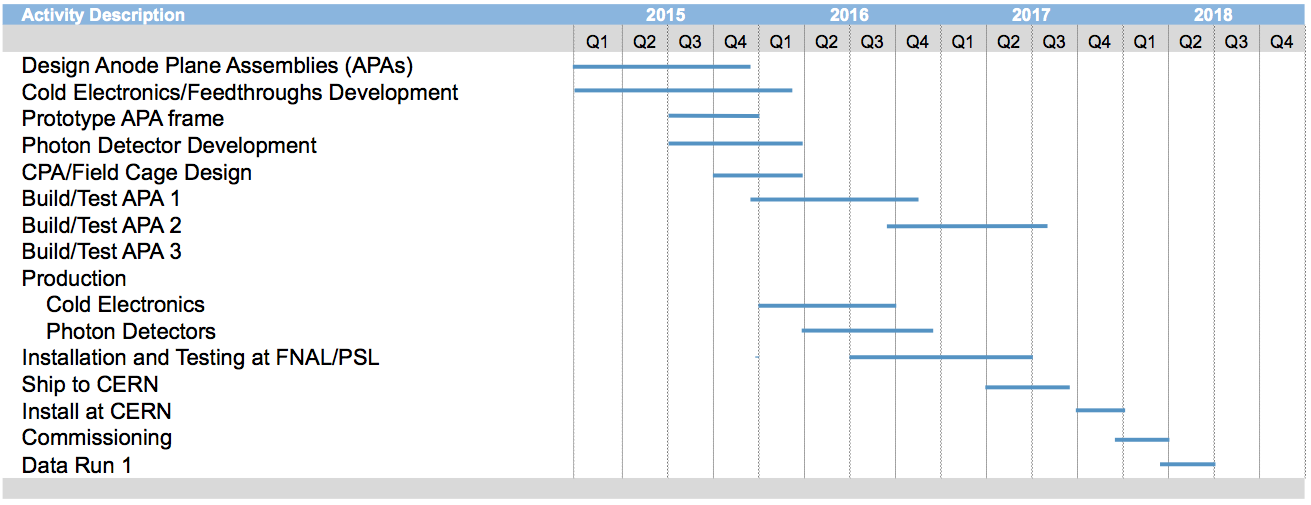
\includegraphics[scale=0.34]{figures/150219_schedule_3APAmod.png}
  \caption{THIS SCHEDULE NEEDS TO BE UPDATED WITH LATEST VERSION!!! Rolled up version of a draft schedule for manufacturing, installing and commissioning the CERN prototype detector. A 2 - 3 months data taking period is included in the schedule. }
  \label{fig:schedule}
\end{figure}


\subsection{Organization}

\begin{itemize}

\item Add description of working group structure 

\end{itemize}



\subsection{Division of Responsibilities}

Work on a MOU between the CERN nu-platform and DUNE describing responsibilities, listing institutions involved and defining deliverables is in progress. The following sections offer an overview of the current plans.

\subsubsection{Shared responsibilities}

The engineering design of the cryostat and the cryogenics system is considered to be a shared responsibility between DUNE/LBNF and CERN.

\subsubsection{DUNE responsibilities}

The following detector components are expected to be covered by the DUNE detector project:
\begin{enumerate}
\item XX APAs
\item CPA
\item field cage
\item cold electronics
\item DAQ hardware and software
\item ...
\end{enumerate}

The following items (incomplete list !) require further discussion. The responsibilities should be clearly spelled out.

\begin{itemize}

\item plans for data analysis and publications:\\
include: description of overlap/commonalities with WA105 data analysis and joined efforts

\end{itemize}




\subsubsection{CERN responsibilities}

\paragraph{The beam line:} design, setup of the beam line and beam monitoring instrumentation are expected to be provided by CERN.

\paragraph{The cryostat and cryogenics system:} are expected to be organized and paid for by the CERN nu-platform.
The scope of the EHN1 cryostat subsystem includes the design, procurement, fabrication, testing, delivery and oversight of a cryostat to contain the liquid argon and the TPC.\\
% moved here from chap 4 (by Anne)

\paragraph{DAQ requests:}  Data links of sufficient bandwidth to transfer the data files from the CENF to the CERN data center, and from there to locations worldwide for analysis. \\

\paragraph{Computing/Software support:} In order to leverage existing software and expertise, appropriate manpower will need to be allocated in order to create and maintain the computing infrastructure necessary for effective use of the reconstruction and physics analysis tools.\\



